\section{Everything-as-a-Service}
\subsection{Was ist XaaS?}
Everything-as-a-Service, auch als XaaS bekannt, ist ein Begriff, der die Bereitstellung einer breiten Palette von Diensten über das Internet beschreibt. Diese Dienste können über herkömmliche webbasierte Anwendungen oder, was häufiger gemeint ist, über modernere cloudbasierte Plattformen bereitgestellt werden. XaaS kann alles umfassen, von Speicher- und Sicherungsdiensten über Software und Anwendungen bis hin zu Infrastruktur- und Plattformdiensten. \cite[vgl.][986f.]{Kollmann.2020} Im Grunde genommen kann jeder Dienst, der über das Internet bereitgestellt werden kann, als XaaS betrachtet werden. Im weitesten Sinne ist auch Human-as-a-Service (HuaaS) miteinbegriffen, also das Nutzen von menschlicher Intelligenz über das Internet wie einen herkömmlichen Webservice. \cite[vgl.][]{CW.2022}
Der Begriff wird im Allgemeinen verwendet, um den Wechsel von herkömmlichen, vor Ort installierten Software- und Hardwarelösungen zu cloudbasierten Lösungen zu beschreiben. Mit XaaS können Unternehmen nur für die Dienste zahlen, die sie benötigen, wenn sie sie benötigen, ohne im Voraus in teure Hardware und Software investieren zu müssen. Der Begriff wird im Allgemeinen verwendet, um den Wechsel von herkömmlichen, vor Ort installierten Software- und Hardwarelösungen zu cloudbasierten Lösungen zu beschreiben. Mit XaaS wird es Unternehmen ermöglicht nur für die Dienste zu zahlen, die sie benötigen, wenn sie sie benötigen, ohne im Voraus in teure Hardware und Software investieren zu müssen. XaaS kann eine kostengünstige Möglichkeit für Unternehmen sein, die benötigten Dienste zu erhalten, ohne in die Infrastruktur zur Unterstützung dieser Dienste investieren zu müssen. Außerdem können Unternehmen dadurch flexibler werden, da sie ihre Dienste je nach Bedarf auf- oder abbauen können.

Klassisch betrachtet, spricht man bei XaaS von drei aufeinander aufbauenden Schichten. Dabei beinhaltet eine Ebene auch immer die Eigenschaften der Darunterliegenden.

\begin{figure}
  \centering
  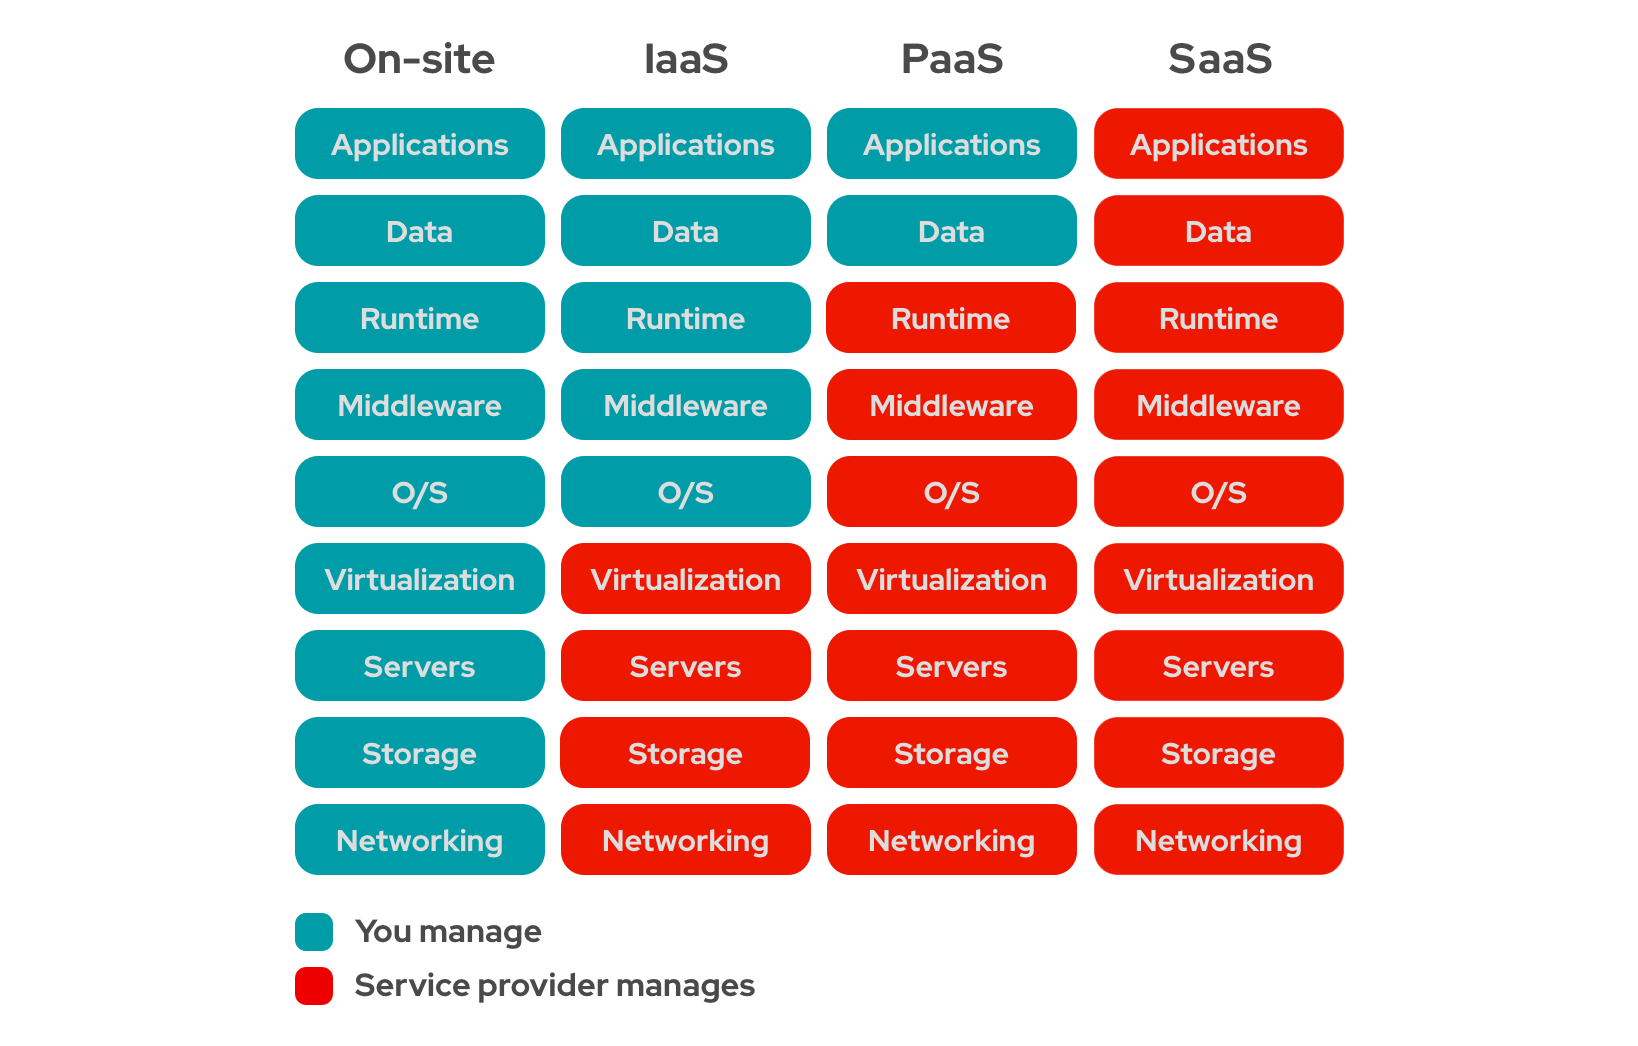
\includegraphics[width=0.9\textwidth]{bilder/xaas.png}
  \caption{Stufenartig aufgebautes Cloud Computing Modell \cite{RedHat.2022}}
  \label{fig:xaasmodell}
\end{figure}


Die drei Hauptkomponenten sind Infrastructure-, Plattform- und Software-as-a-Service. Wie in der Abbildung zu sehen ist kommen bei jeder Stufe im Gegensatz zu dem klassischen On-Site-Ansatz, bei dem jegliche Infrastruktur selbst beschafft und vor Ort gehostet wird, Services dazu, die die Service Provider verwalten und nicht mehr selbst gemanaged und gewartet werden müssen. \cite[vgl.][]{RedHat.2022}


\subsection{Infrastructure-as-a-Service (IaaS)}
Infrastructure-as-a-Service ist die unterste Ebene des dreischichtigen Servicemodells von Cloud Computing. Man versteht darunter das Modell, bei dem ein Drittanbieter eine Computerinfrastruktur als Dienst anbietet. Das heißt, bei IaaS wird das Hosting geoutsourced, wobei der IaaS-Kunde nicht der Eigentümer der Infrastruktur ist, sondern diese bei einem Provider mietet. Die IaaS-Anbieter stellen diese Ressourcen dann auf Abruf aus ihren umfangreichen, in Rechenzentren installierten Gerätepools bereit. Dieser ist dann auch für die Wartung und den Support der Hardware und Software verantwortlich, so dass sich der Kunde auf sein Kerngeschäft konzentrieren kann. Die Kunden zahlen nur für die Menge an Rechen-, Speicher- und Netzwerkressourcen, die sie nutzen, in der Regel auf einer Pay-as-you-go-Basis. Dies steht im Gegensatz zum traditionellen Modell des Kaufs und der on-premise Verwaltung von Hardware und Software, die kapitalintensiv sein können und erhebliche laufende Wartungs- und Supportkosten erfordern.

Zusammenfassend lässt sich sagen, dass IaaS ein Cloud-Computing-Modell ist, das es Unternehmen ermöglicht, das Hosting und die Wartung ihrer Hardware- und Software-Ressourcen auszulagern. Es bietet Unternehmen die Möglichkeit, Ressourcen schnell und bedarfsgerecht zu skalieren, auf die neuesten Technologien zuzugreifen, ohne in teure Hardware- und Software-Upgrades investieren zu müssen, und individuelle Lösungen für ihre spezifischen Anforderungen zu entwickeln. \cite[vgl.][31]{HuaweiTechnologies.2023} \\


\subsection{Platform-as-a-Service (PaaS)}
Die nächste Ebene im Cloud Computing Modell ist Platform-as-a-Service oder auch PaaS. PaaS-Anbieter bieten eine Umgebung an, in der Anwendungen entwickelt, ausgeführt und verwaltet werden können, ohne dabei die zugrundeliegende Infrastruktur aufbauen zu müssen. PaaS-Dienste ermöglichen es den Benutzern, über eine Internetverbindung auf eine Plattform und alle zugehörigen Dienste zuzugreifen, wodurch die Installation, Konfiguration und Verwaltung von Hardware und Software entfällt. Dies kann die Kosten senken und den Entwicklungsprozess beschleunigen. PaaS-Dienste umfassen in der Regel Betriebssysteme, Webserver, Anwendungsserver, Datenbanken, Speicherdienste und andere Dienste zur Erstellung und Bereitstellung von Anwendungen. \\
Zusammenfassend spricht man bei PaaS häufig auch von einem ,,Cloud-Betriebssystem``. PaaS kann für die schnelle Entwicklung und Bereitstellung von Webanwendungen, mobilen Anwendungen und anderen Softwareanwendungen verwendet werden, ohne dass dabei die Komplexität der Verwaltung der zugrundeliegenden Infrastruktur auf sich genommen werden muss. \cite[vgl.][31ff.]{HuaweiTechnologies.2023} \\


\subsection{Software-as-a-Sercice (SaaS)}
Auf der obersten Ebene des dreistufigen Cloud Computing Modells und somit die umfangreichste Bereitstellung von Diensten ist Software-as-a-Service oder auch SaaS. SaaS ist eine Softwarebereitstellungsmethode, bei der die gesamte Software, also inklusive Infrastruktur und Betriebssystem, auf entfernten Servern zentral gehostet wird und die Nutzer über das Internet mit einem standard Webbrowser darauf zugreifen können. SaaS-Anwendungen werden manchmal auch als webbasierte Software, On-Demand-Software oder gehostete Software bezeichnet. Mit SaaS können die Kunden von jedem Ort, zu jeder Zeit und mit jedem Gerät, das über eine Internetverbindung verfügt, auf die Software zugreifen, ohne die Software auf ihren eigenen Servern oder Geräten installieren und verwalten zu müssen. SaaS-Lösungen sind in der Regel abonnementbasiert und werden auf monatlicher oder jährlicher Basis bezahlt. \\

Diese Dienste sind sowohl für allgemeine Nutzer (Anwendungen wie Google Calendar und Gmail), als auch für Unternehmensgruppen zur Unterstützung von Gehaltsabrechnungen, Personalverwaltung, und für die Verwaltung von Kunden- und Geschäftspartnerbeziehungen. Durch diese Anwendungen wird der Zeitaufwand für die Installation und Wartung der Software reduziert und es muss auch keine Hardware, Software und spezielles IT-Personal beschafft werden. \cite[vgl.][33f.]{HuaweiTechnologies.2023} \\

